\section{A3.3}
\subsection{a)}
Plop is a function, that takes an empty list and some value and insert that value into the list.
In the "second" line plop is called with a list pattern and the argument w. And then insert U and V in the start of the list and then
insert w at the end of the instantiated list.

\subsection{b)}
% \begin{figure}[H]
%     \centering
%     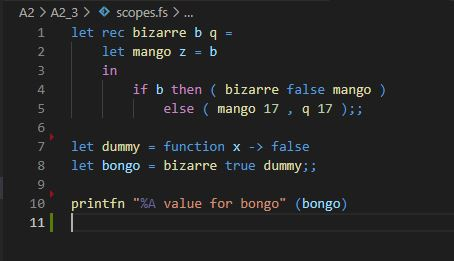
\includegraphics[width=0.75\textwidth]{Figures/Scope_rules.JPG}
%     \caption{Modified F\# code from assignment text}
% \end{figure}
